\documentclass[10pt]{article}

\usepackage{ucs}
\usepackage[utf8x]{inputenc}
\usepackage[english]{babel}
\usepackage{fontenc}
\usepackage{graphicx}

\usepackage[dvips]{hyperref}

\author{Carson Holgate}
\title{Adiabatic Quantum Computation\\ at D-Wave Systems Inc.}
\date{05/10/2010}


\begin{document}
\maketitle

\paragraph{Adiabatic Quantum Computation}

as the name implies--relies on the adiabatic theorem to make computations. In 1928 Max Born and Vladimir Fock stated the theorem as follows: 
  \begin{quote}
   A physical system remains in its instantaneous eigenstate if a given perturbation is acting on it slowly enough and if there is a gap between the eigenvalue and the rest of the Hamiltonian's spectrum.
  \end{quote}
As it applies to quantum computation, if a non-degenerate system is initialized in the ground state 
  \[|\psi(0)\rangle\] 
of a given Hamiltonian 
  \[\mathcal{H}(0)\] 
and is allowed to evolve slowly according to the Schr\"{o}dinger equation 
  \[ i \frac{d}{dt} |\psi(t)\rangle = \mathcal{H}(t)|\psi(t)\rangle\] 
then as long as there is a non-zero energy gap between \(|\psi(0)\rangle\) and the next lowest energy state, \(|\psi(t)\rangle\) will remain close to the ground state of \(\mathcal{H}(t)\) at any given time.

Because it relies on the evolution of the state of a system, adiabatic quantum computation does not involve gates.   Instead, the solution to a given problem is encoded in the ground state of a problem Hamiltonian 
  \[\mathcal{H}_P\] 
It is generally easy to find \(\mathcal{H}_P\) but difficult to find the ground state. To complete the system an initial Hamiltonian 
  \[\mathcal{H}_B\] 
with an easily solvable ground state is chosen.  The system is described by both Hamiltonians as:  
  \[\mathcal{H}(t) = (1-t/T)\mathcal{H}_B + (t/T)\mathcal{H}_P\] 
Where T is a parameter to control the rate at which \(\mathcal{H}(t)\) varies.  Normalized to \(\tilde{\mathcal{H}}(s), 0 \leq s\leq 1\): 
  \[\tilde{\mathcal{H}}(s) = (1-s)\mathcal{H}_B + s\mathcal{H}_P\]
At this point the system is initialized to the ground state \(|\psi(0)\rangle\) where 
  \[\tilde{\mathcal{H}}(0) = \mathcal{H}_B\] 
and after sufficient time evolution \(|\psi(t)\rangle\) becomes the ground state of \(\mathcal{H}_P\)

\paragraph{D-Wave}
is the first company to develop a functional adiabatic quantum computer.  It was founded in 1999 by: 
  \begin{itemize}
   \item Haig Farris
   \item Geordie Rose (CTO)
   \item Bob Wiens (former CFO)
   \item Alexandre Zagoskin (Chief Scientist)
  \end{itemize}
and was started as an off-shoot of the University of British Columbia funding academic research in quantum computing.  

The company was founded with the goal of finding a way--with existing fabrication techniques--to solve a specific set of NP hard problems known as Quadratic Unconstrained Binary Optimization (QUBO) problems which are common in pattern matching problems and machine learning applications.  QUBO problems are equivalent to finding the lowest energy states of the two dimensional classical Ising Hamiltonian: 
  \[\mathcal{H} = \displaystyle\sum\limits_{i}h_i\sigma_{zi} + \displaystyle\sum\limits_{ij}J_{ij}\sigma_{zi}\sigma_{zj}\]

D-Wave accomplished this with a Superconducting Quantum Interference Device (SQUID) based flux qubit system:
 \begin{center}
  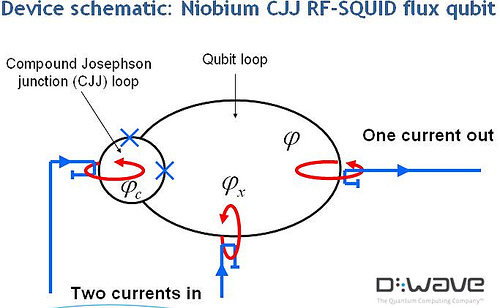
\includegraphics[scale=.7]{../img/Qubit_Schematic}
 \end{center}
which operates on low power at ultra low temperatures and has been manufactured at NASA's Jet Propulsion Laboratories.  This system uses a method similar to simulated annealing to solve QUBO problems which results in good solutions but not necessarily the best solution to any given problem. 

In 2007 D-Wave demonstrated example pattern matching on Orion, their 16-qubit system powered by the Chimera C4 chip.  Since then they have been working with Google on imaged based image search for applications like Google Goggles that makes use of vector matching, and on machine learning to recognize cars for vehicle safety systems.  D-Wave recently released early access to an API for Orion web services to allow users to submit programs to run on the quantum server.  Currently the web service back-ends to a server that simulates the Orion system but the actual quantum system should be up and running eventually.

\paragraph{Controversy} exists as to whether or not Orion is a real quantum computer.  D-Wave has published unconfirmed reports of a speed up in processing time but skeptics attribute it to the super conducting materials.  Orion conforms to some of the Vincenz criteria for quantum computers but not all:
  \begin{enumerate}
  \item A scalable physical system with well characterized qubits
  
  While the qubits are well characterized, scalability is a problem with Orion.  To have a truly fully entangled system, every qubit must be physically connected to every other qubit.  To make each these connections additional hardware and length must be added to a qubit which adds energy and instability to the system.
  \item The ability to initialize state

  Control circuitry for each qubit along with super cooling allows for initialization.

  \item Long relevant decoherence times

  SQUID flux qubits have long decoherence times.

  \item Universal set of quantum gates
  
  Adiabatic quantum computers do not rely on quantum gates.  Aharonov, van Dam, et al. proved that adiabatic quantum computation is equivalent to standard quantum computation preformed on experimental Nuclear Magnetic Resonance systems.

  \item The ability to measure specific qubits

  Individual qubits can be easily measured.

 \end{enumerate}

Further controversy surrounds the problems targeted by Orion.  A subset of QUBO problems are NP-Complete; one of the fundamental characteristics of NP-Complete problems is that every NP-Complete problem can be reduced to every other NP-Complete problem.  Goldman, Gutmann, and Sipser published an adiabatic algorithm to solve 3-SAT, a well known NP-Complete problem.  Theoretically it should also be possible to solve all NP-Complete problems with an adiabatic quantum computer but because Orion uses simulated annealing techniques it does not produce exact results and therefore does not solve NP-Complete problems.

\bigskip 
The corresponding presentation can be found online: {\em http://github.com/clholgat/MA591-DWave }


  \begin{thebibliography}{10}
 
  % Followed by interesting articles. Keep the list short. 
  \bibitem{AQC=SQC2005}
    D.~Aharonov, W.~vanDam, J.~Kempe, Z.~Landau, S.~Lloyd, O.~Regev
    \newblock Adiabatic Quantum Computation is Equivalent to Standard Quantum Computation.
    \newblock {\em arXiv:quant-ph/0405098v2},2005.
  
  \bibitem{PIQC2000}
    D.~Vincenz.
    \newblock The Physical Implementation of Quantum Computation.
    \newblock {\em arXiv:quant-ph/0002077v3},2000.

  \bibitem{AQC2000}
    E.~Farhi, J.~Goldstone, S.~Gutmann, M.~Sipser
    \newblock Quantum Computation by Adiabatic Evolution.
    \newblock {\em arXiv:quant-ph/0001106v1},2000.

  \bibitem{RSFQ2009}
    R.~Harris et al.
    \newblock Experimental Demonstration of a Robust and Scalable Flux Qubit
    \newblock {\em arXiv:0909.4321v1 [cond-mat.supr-con]},2009.

  \bibitem{GRB2009}
    H.~Neven
    \newblock Machine Learning with Quantum Algorithms
    \newblock {\em http://googleresearch.blogspot.com/2009/12/machine-learning-with-quantum.html},2009.

  \bibitem{GRBlog2010}
    G.~Rose
    \newblock rose.blog
    \newblock {\em http://dwave.wordpress.com/}

  \bibitem{GTT2007}
    H.~Neven, G.~Rose
    \newblock Google Tech Talks: Quantum Computing
    \newblock {\em http://www.youtube.com/watch?v=I56UugZ_8DI&feature=channel},2007.

  \bibitem{dwavesite2010}
    \newblock D-Wave Systems Inc.
    \newblock {\em http://www.dwavesys.com/}


  \end{thebibliography}



\end{document}

